\subsubsection{Pautas de fase e projeto}

No página de gestão de um projeto, um aluno pode consultar uma pauta detalhada. Esta pauta lista todos os alunos inscritos na unidade curricular associada ao projeto e respetiva nota.

Além da nota final do projeto, também é possível ver a nota de cada fase.

Na Figura~\ref{fig:student_grades_project} pode ser consultada uma imagem demonstrativa da página desenvolvida.

\begin{figure}[H]
	\centering
	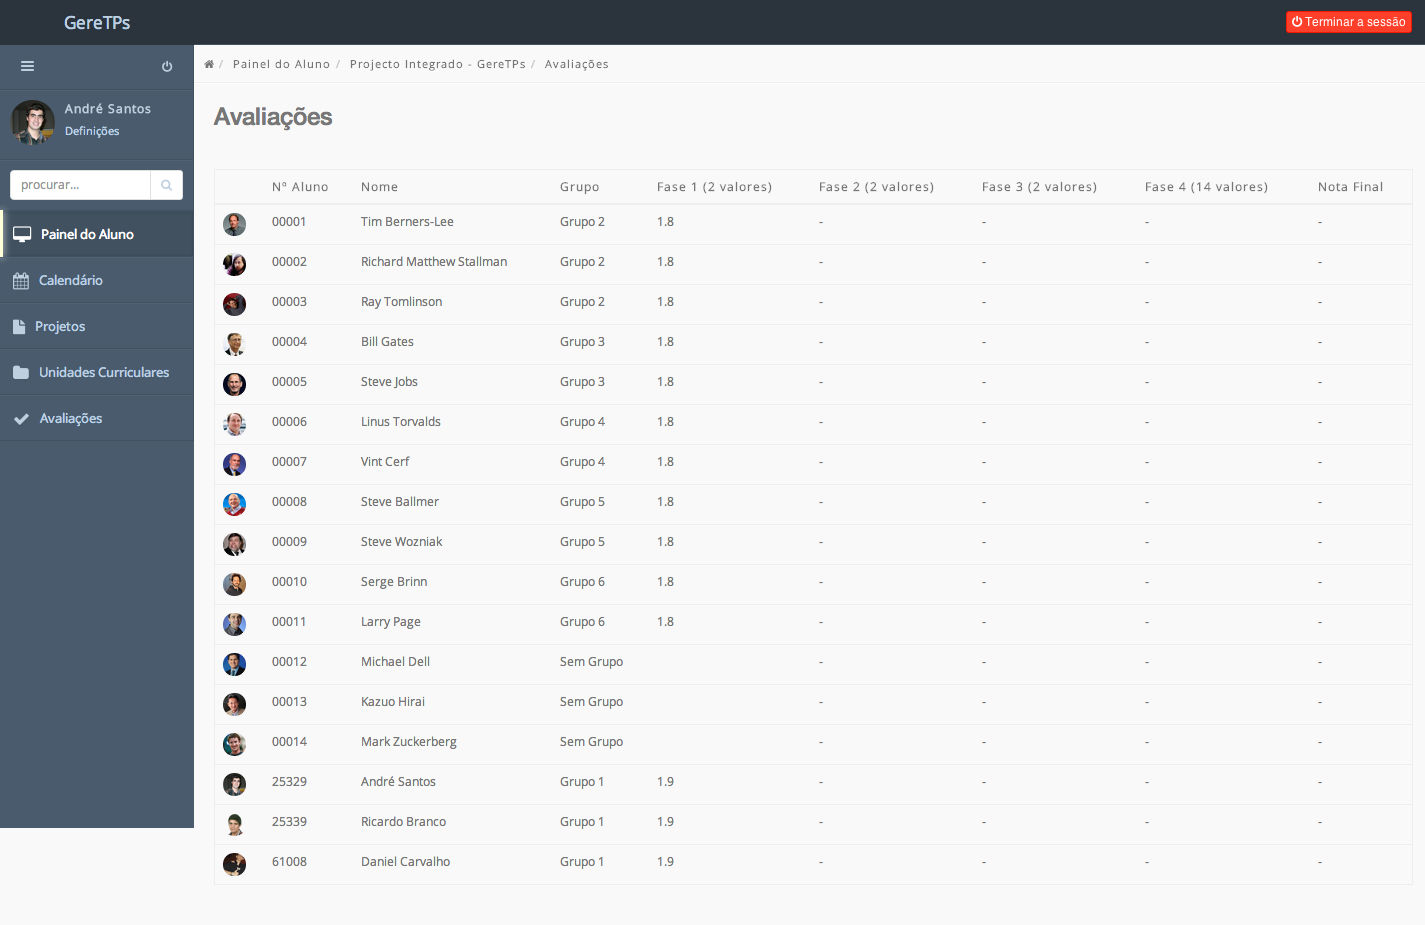
\includegraphics[width=1\textwidth,center]{images/implementacao/alunos/grades_project}
	\caption{Pauta de um projeto}
	\label{fig:student_grades_project}
\end{figure}

Ainda na página de gestão de um projeto, é possível aceder à página de \hyperref[ssub:gestao_fases]{Gestão de fases e entregas}. A partir desta página é possível um aluno consultar a pauta de uma fase de um projeto, caso esta já tenha sido lançada por um dos docentes da unidade curricular associada ao projeto.

A pauta de uma fase é bastante semelhante à pauta de um projeto, com a particularidade de esta apresentar a nota da fase entre zero e vinte valores e a nota correspondente no final do projeto.

Na Figura~\ref{fig:student_grades_phase} pode ser consultada uma imagem demonstrativa da página desenvolvida.

\begin{figure}[H]
	\centering
	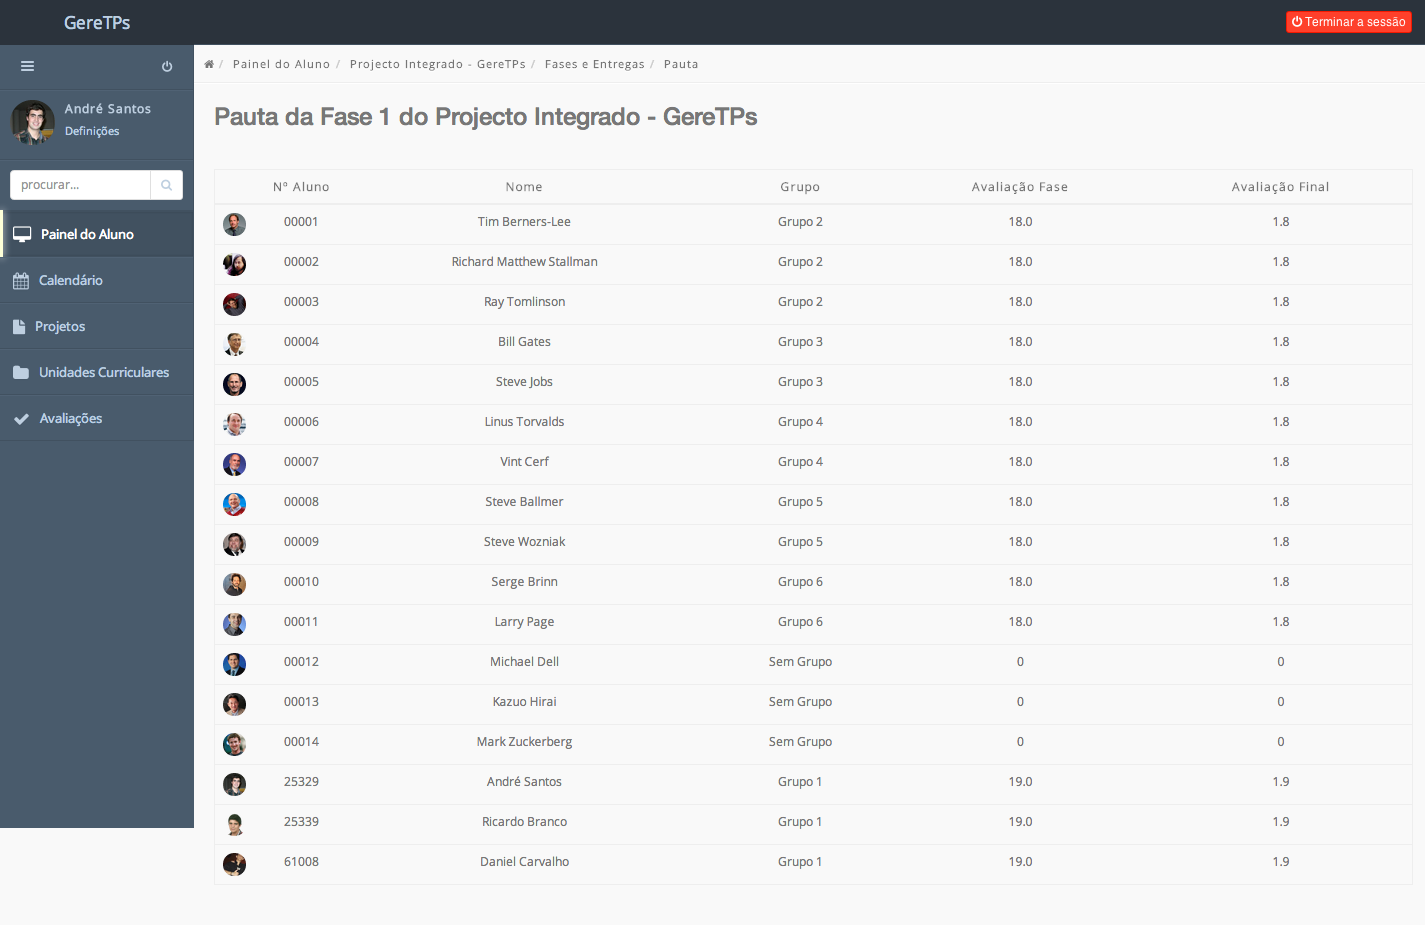
\includegraphics[width=1\textwidth,center]{images/implementacao/alunos/grades_phase}
	\caption{Pauta da uma fase}
	\label{fig:student_grades_phase}
\end{figure}
